\chapter{Integrali Doppi e tripli}
\section{Domini normali (semplici)}
\begin{defi}
	I domini delle funzioni a più variabili possono presentare una forma di
	regolarità per cui è possibile delimitare la regione da intervalli e grafici
	di funzione. Si parla quindi di dominio semplice o normale rispetto alla
	variabile delimitabile da un intervallo. La normalità di un dominio è molto
	importante in molte definizioni di integrale multiplo e della sua
	risoluzione tramite le formule di riduzione. Inoltre la presenza di un
	dominio regolare permette ulteriori teoremi e formule d'integrazione, come
	le formule di Gauss-Green, il teorema della divergenza e il teorema del
	rotore.
\end{defi}
\subsection{Dominio normale rispetto all'asse $x$}
Il dominio A si definisce {\color{red} normale} rispetto all'asse $x$ se è così
definito:
\begin{equation}
	A=\begin{cases}
		a\leq x\leq b & x \text{ valria in un intervallo}\\
		g_1(x)\leq y\leq g_2(x) & y \text{ varia tra due funzioni di }x
	\end{cases}
\end{equation}
\begin{esempio}
\begin{equation*}
	D=\begin{cases}
		0\leq x\leq 1\\
		x^2\leq y\leq x
	\end{cases}
\end{equation*}
\end{esempio}
Il dominio $B$ si definisce {\color{red} normale} rispetto all'asse $x$ se è così
definito:
\begin{equation}
	A=\begin{cases}
		c\leq y\leq d & y \text{ valria in un intervallo}\\
		h_1(y)\leq x\leq h_2(y) & x \text{ varia tra due funzioni di }y
	\end{cases}
\end{equation}
\begin{esempio}
\begin{equation*}
	D=\begin{cases}
		0\leq y\leq 1\\
		y< x< \sqrt{y}
	\end{cases}
\end{equation*}
\end{esempio}
\subsection{Domini Polarmente normale}
Il dominio C si definisce polarmente normale se è costantemente definito:
\begin{equation}
	C=\begin{cases}
		\theta_1\leq \theta\leq \theta_2 \\
		\varphi_1(\theta)\leq \varphi(\theta)\leq \varphi_2(\theta)
	\end{cases}
\end{equation}
\begin{esempio}
  \begin{equation}
    (x-1)^2+y^2\leq 1
  \end{equation}
  l'angolo varia tra 0 e $\frac{\pi}{2}$, il segmento $\varphi$ dipende dall'angolo
  \begin{equation*}
    \begin{matrix}
      \theta=0\text{ è } \max \varphi=2 \\
      \theta=\frac{\pi}{2} \text{ è } \min \varphi=0 \\
      \varphi=2\cos \theta
      \begin{cases}
        0\leq \theta \leq \frac{\pi}{2}\\
        0\leq \varphi\leq 2\cos \theta
      \end{cases}
    \end{matrix}
  \end{equation*}
  corona circolare $\varphi=r$ $\varphi=R$
  \begin{equation*}
    \begin{cases}
      0\leq \theta \leq \frac{\pi}{2}\\
      r\leq \varphi\leq R
    \end{cases}
  \end{equation*}
\end{esempio}
\subsection{Definizione di integrale doppio}
\begin{defi}
  Sia f(x,y) una funzione limitata nel rettangolo $R=[a,b]x[c,d]$, coordinata in $[a,b]$ e
  di seconda coordinata in $[c,d]$
  Deconpongo regolarmante gli intervalli $[a,b]$ e $[c,d]$,
  \begin{equation*}
    \begin{matrix}
        \text{decomponendo }[a,b]\text{ si ha} & D_1=\{x_0=a,x_1,x_2,\dots,x_n=b\}\\ 
        \text{decomponendo }[c,d]\text{ si ha} & D_1=\{y_0=a,y_1,y_2,\dots,y_n=d\}
    \end{matrix}
  \end{equation*}
  Il prodotto cartesiano $D=D_1*D_2$ è una semidivisione del rettangolo R
  \begin{figure}[ht]
    \centering
    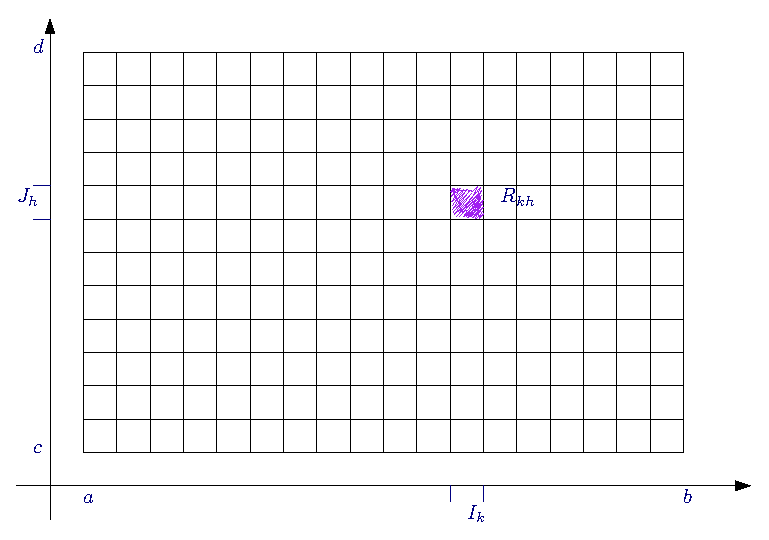
\includegraphics[width=8cm]{img/finiti/graficodecomposizioneR.eps}
    \caption{Decomposizione del rettangolo R}
  \end{figure}
  \begin{equation*}
    \begin{matrix}
        I_k=[x_{k-1},x_k] \text{ in } D_1 (k=1,\dots,n)\\
        J_h=[y_{h-1},y_h] \text{ in } D_2 (h=1,\dots,n)
    \end{matrix}
  \end{equation*}
  Il prodotto cartesiano $I_k*J_h$ individua il generico subrettangolo $R_{kh}$ della semidivisione.\\
  Prendo un generico punto del subrettangolo $R_{kh}(x_k,y_h)$ e faccio il seguente prodotto:
  \begin{equation*}
    f(x_k,y_h)*mis R_{kh} \text{ con } misR_{kh} = misI_k * misJ_h \text{ area del subrettangolo}
  \end{equation*}
  Con l'integrale doppio consudero il volume del parallelepipedo.\\
  Geometricamente considera il pettangolo $R_{kh}$ e la parte di superficie $f(x,y)$ che vi si
  presenta il prodotto $f(x_i,y_n)*mis R_{kh}$ è il volume del parallelepipedo di base $R_{kh}$
  e altezza $f(x_k,y_h)$.
\end{defi}
\section{Somme di Riemann}
Definisco le somme di Riemann $\displaystyle\sum^{k=m\text{ } h=n}_{k=h=1}f(x_k,y_h)*R_{kh}$ ciò
rappresenta la somma di tutti i volumi dei parallelepipedi di base $R_{kh}$ e altezza $f(x_k,y_h)$
che si possono ottenere nel rettangolo $R$.\\
Infittisco le decomposizioni $D_1$ e $D_2(m\to \infty;n\to\infty)$, ottenendo così un numero sempre
maggiore di subrettangoli di ampiezza via via minore.
\begin{equation}
  mis R_{kn}=misI_k*misI_n=\frac{b-a}{m} * \frac{d-c}{n}\to 0 \text{ per }  m,n \to \infty
\end{equation}
Con l'infittirsi della decomposizione, aumenta la precisione con cui ciascun parallelepipedo
approssima il volume sotto al grafico delle funzione in ogni $R_{kh}$.\\
Al limite, le somme di Riemann daranno il volume sotto al grafico della funzione in un certo
rettangolo (in generale dominio).\\
Se esiste finito $\lim\limits_{n\to \infty\text{ } m\to \infty}\displaystyle\sum_{h=k=1}^{k=m\text{ }h=n}f(x_k.y_n)*misR_{kh}$ tale limite è definito \underline{\color{red} ingrale doppio} di f(x,y) nel
dominio $R=[a,b]*[c,d]$
\begin{equation}
  \iint_R f(x,y)dxdy=\lim\limits_{n\to \infty\text{ } m\to \infty}\displaystyle\sum_{h=k=1}^{k=m\text{ }h=n}f(x_k.y_n)*misR_{kh}
\end{equation}
\paragraph{Somme superiori e somme inferiori}
\begin{defi}
  È possibile definire l'integrale doppio anche con le somme superiori e le somme inferiori
  \begin{equation*}
    \text{Somme inferiori } s(f,R) = \displaystyle\sum inf_{R_{kh}}f(x_k.y_n)*misR_{kh}
  \end{equation*}
  prendo il minimo valore che la funzione assume nel subrettangolo $R_{kh}$ e lo moltiplico per
  l'area di tale subrettangolo. Sommando ottengo un parallelepipedo, il cui volume approssima
  per difetto individuato dalla funzione. 
  \begin{equation*}
    \text{Somme superiori } s(f,R) = \displaystyle\sum sup_{R_{kh}}f(x_k.y_n)*misR_{kh}
  \end{equation*}
  prendo il massimo valore che la funzione assume nel subrettangolo $R_{kh}$ e lo moltiplico per
  l'area di tale subrettangolo. Sommando ottengo un parallelepipedo, il cui volume approssima per
  eccesso quello individuato dalla funzione all'infittirsi della decomposizione le somme inferiori
  crescono, le somme superiori decrescono. Le somme superiori e le somme inferiori convergono ad
  uno stesso valore, detto {\color{red}integrale doppio}\footnote{è il valore sotto al grafico
    della funzione}
  \begin{equation*}
    \lim s=\lim S=\iint_R f(x,y)dxdy
  \end{equation*}
\end{defi}
\clearpage
\subsection{Proprietà dell'integrale doppio}
\begin{equation*}
  \begin{matrix}
  \text{Linearità } \begin{cases}
                      1) \iint_D [f_1(x,y)+f_2(x,y)]dxdy=\iint_Df_1(x,y)dx*dy+\iint_Df_2(x,y)dx*dy\\
                      2) \iint_D \alpha f_1(x,y)dxdy=\alpha\iint_Df_2(x,y)dx*dy
                    \end{cases}\\
    \text{Assitività } 3)\text{ Sia } D=D_1\cup D_2 \iint_Df(x,y)dxdy=\iint_{D_1}f(x,y)dx*dy +\iint_{D_2}f(x,y)dx*dy\\
    \text{Monotonia } \begin{cases}
                        4) \text{ Sia } f(x,y)\leq g(x,y)\text{ } \forall (x,y) \in D\\
                        \text{ }\iint_Df(x,y)dxdy \leq \iint_Dg(x,y)dx*dy\\
                        5) \text{ Sia } D_1 \subset D\\
                        \text{ } \iint_{D_1}f(x,y)dxdy < \iint_Df(x,y)dx*dy \\
                        6) \abs{\iint_Df(x,y)dxdy} \leq \iint_D\abs{f(x,y)}dx*dy
                      \end{cases}
  \end{matrix}
\end{equation*} 

\subsection{Formula di riduzione}
\begin{itemize}
\item Sia $A\subset R^2$ un dominio normale rispetto all'asse x
  \begin{equation*}
    A=\begin{cases}
        a\leq x\leq b\\
        g_1(x)\leq y\leq g_2(x)
      \end{cases}
  \end{equation*}
    Allora $\iint_A f(x,y) dxdy=\int_a^bdx \left(\int_{g_1(x)}^{g_2(x)}f(x,y)dy\right)$\\
    calcolo prima $\int_{g_1(x)}^{g_2(x)}f(x,y)dy$ che è una funzione della sola $x$ $\not{o}(x)$
    \begin{equation*}
      \text{per calcolo } \int^b_a \not{o} (x) dx
    \end{equation*}
  \item Dominio polarmente normale\\
    Effettua un cambio di coordinate, passando dalle coordinate cartesiane a quelle polari
    \begin{equation*}
      \text{L'integrale doppio è } \iint_Df(x,y)dxdy
    \end{equation*}
    Passando alle coordinate polari
    \begin{equation*}
      \begin{matrix}
        \text{del dominio } D(x,y) \text{ passerò al dominio } D^\prime (\varphi, \theta) \\
        \text{della funzione } f(x,y) \text{ passerò al dominio } f (\varphi, \theta)
      \end{matrix} \begin{cases}
                       x=\varphi\cos\theta\\
                     y=\varphi\sin\theta
                   \end{cases}
                   \varphi=\sqrt{x^2+y^2} 
   \end{equation*}
   e da differenziali $dxdy$ passerò ai differenziali $d\varphi d\theta$. \\
   Si dimostra che nel passaggio ad altre coordinate il differenziale è $\abs{j} d\varphi d\theta$,
   dove $\abs j$ è il determinante della {\color{red} matrice Jacobiana} che contiene le derivate
   parziale prime
   \begin{equation}
     \abs{J}=\begin{vmatrix}
               x_\varphi & x_\theta\\
               y_\varphi & y_\theta
             \end{vmatrix}
             \to \abs{J}=\begin{vmatrix}
                           \cos \theta & -\varphi \sin \theta\\
                           \sin \theta & \varphi \cos \theta
                         \end{vmatrix}
                         =\varphi\cos^2\theta+\varphi \sin^2\theta =\varphi
   \end{equation} 
   Per cui passando da $dxdy$ alle coordinate polari avrò $\varphi d\varphi d\theta$ così
   l'integrale doppio diventa:
   \begin{equation*}
     \iint_Df(x,y)dxdy=\iint_{D^\prime}f(\varphi,\theta)\varphi d\varphi d\theta
   \end{equation*}
\end{itemize}
\clearpage
\subsubsection{Esempi di domini polarmente normali}
\begin{figure}[ht]
  \centering
  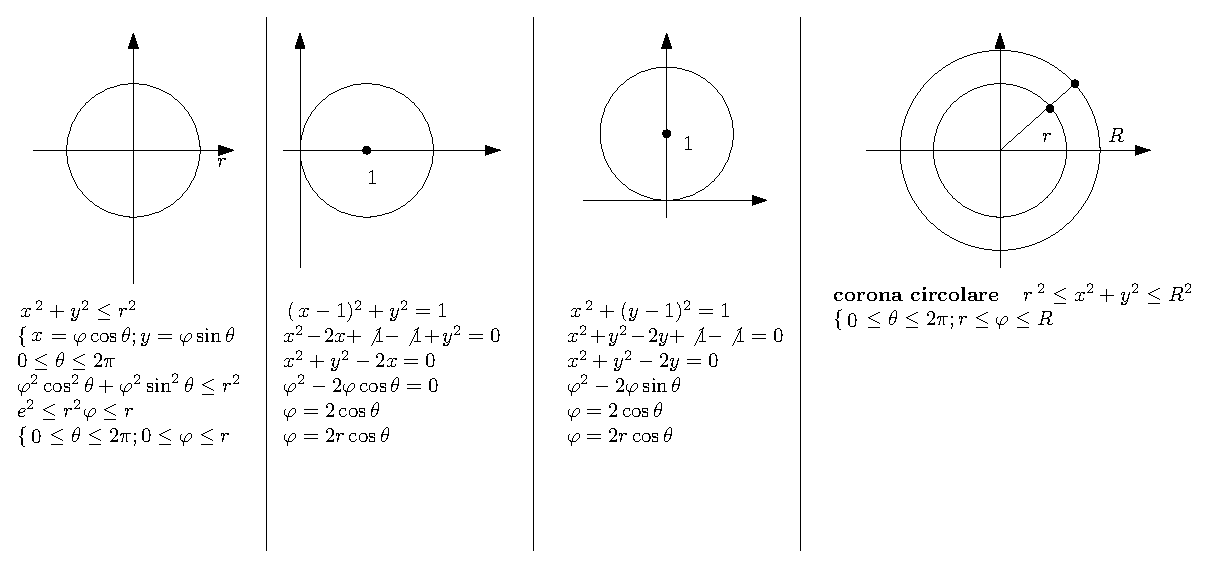
\includegraphics[width=14cm]{img/finiti/esdompolnorm.eps}
  \caption{Esempi di domini polarmente normali}
\end{figure}
\subsection{Baricentro di un dominio normale}
\begin{defi}
  Sia D un demonio normale del piano. Si definisce {\color{red}baricentro del dominio} D il punto di
  coordinate $(x_0,y_0)$ tale che:
  \begin{equation*}
    \begin{matrix}
      x_0=\frac{1}{mis D} \iint_D xdxdy & y_0=\frac{1}{mis D} \iint_D ydxdy
    \end{matrix}
  \end{equation*}
  $mis D:$ misura ({\tt area}) del dominio $D$.
\end{defi}
\begin{esempio}
  calcolare il baricertro del dominio $D=\begin{cases}
                                           0\leq x\leq 2\\
                                           0\leq y\leq 1
                                         \end{cases}$
  \begin{equation*}
    mis D=A_{rettangolo}=2*1=2
  \end{equation*}
  \begin{figure}[ht]
    \centering
    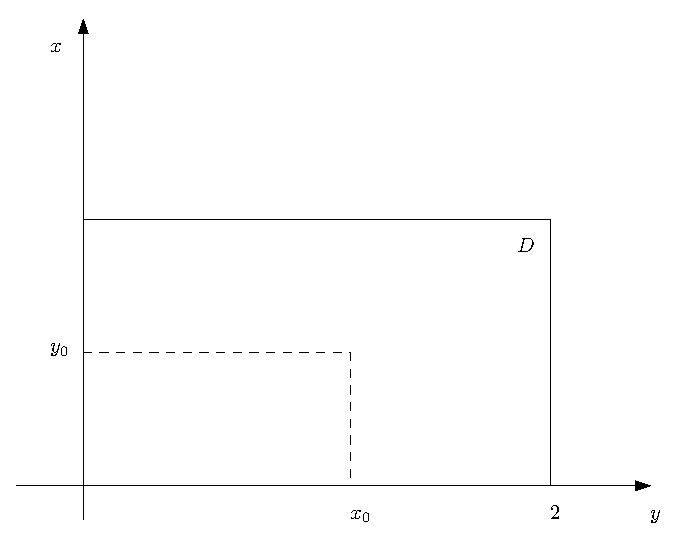
\includegraphics[width=6cm]{img/finiti/baricentrodiundominionormale.eps}
    \caption{Baricentro di un dominio normale}
  \end{figure}
  \begin{equation*}
    \begin{matrix}
      x_0=\frac{1}{mis D}\iint_D xdxdy=\frac{1}{2}\int_0^2dx\int_0^1xdy=\frac{1}{2}\int^2_0dx\abs{xy}_0^1= \frac{1}{2}\int_0^2xdx=\frac{1}{2}\abs{\frac{x^2}{2}}_0^2=\frac{1}{\not{2}}\not{2}=1\\
      y_0=\frac{1}{mis D}\iint_D ydxdy=\frac{1}{2}\int_0^2dx\int_0^1ydy=\frac{1}{2}\int_0^2dx\left|\frac{y^2}{2}\right|^1_0=\frac{1}{2}\int^2_0\frac{1}{2}dx=\frac{1}{4}\left|x\right|=\frac{1}{2}
    \end{matrix}
  \end{equation*}
  \clearpage
   \begin{center}
            \fbox
            {
            \begin{minipage}{0.85\textwidth}
		Calocolare il baricentro del dominio $D=\begin{cases}
                                                          0\leq \theta \leq \frac{\pi}{2}\\
                                                          0\leq y \leq \sqrt{1-x^2}
                                                          \end{cases}$
              \begin{multicols}{2}
                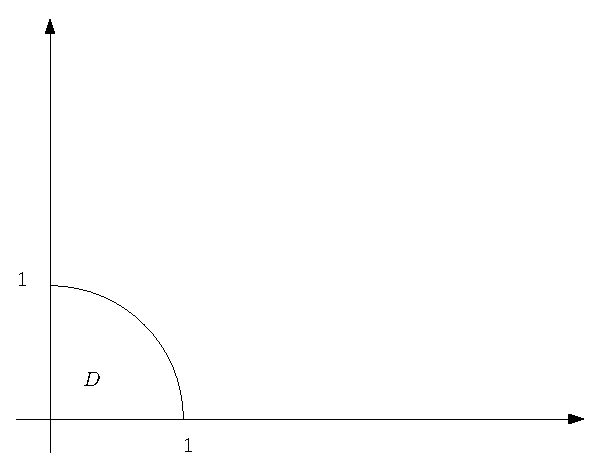
\includegraphics[width=6cm]{img/finiti/baricentrodiundominionormale2.eps}\\
                \begin{equation*}
                  \begin{matrix}
                    D=\begin{cases}
                      0\leq \theta\leq\frac{\pi}{2}\\
                      0\leq \varphi\leq 1
                    \end{cases} & mis D=\frac{\pi}{4}
                  \end{matrix}
                \end{equation*}
              \end{multicols}
              \begin{equation*}
                \begin{matrix}
                  x_0= \frac{1}{mis D}\iint_D xdxdy=\frac{4}{\pi}
                  \int^{\frac{\pi}{2}}_0d\theta\int_0^1
                  \varphi^2\cos \theta d\theta = \frac{4}{\pi} \int_0^{\frac{\pi}{2}}d\theta \left|
                  \frac{\varphi^3}{3}\cos\theta\right|_0^1\\=\frac{4}{\pi}\int_0^{\frac{\pi}{2}}
                  \frac{1}{3} \cos \theta d\theta = \frac{4}{3}\pi \left|\sin
                  \theta\right|^{\frac{\pi}{2}}_0=\frac{4}{3}\pi\\
                  y_0=\frac{1}{mis D}\iint_D xdxdy=\frac{4}{\pi}
                  \int^{\frac{\pi}{2}}_0d\theta\int_0^1
                  \varphi^2\sin \theta d\theta = \frac{4}{\pi} \int_0^{\frac{\pi}{2}}d\theta \left|
                  \frac{\varphi^3}{3}\sin\theta\right|_0^1\\
                  =\frac{4}{\pi}\int_0^{\frac{\pi}{2}}\frac{1}{3}\sin\theta d\theta =\frac{4}{\pi}*
                  \frac{1}{3}\left|-\cos\theta \right|^{\frac{\pi}{2}}_0=\frac{4}{3}\pi
                \end{matrix}
              \end{equation*} 
            \end{minipage}
            }
  \end{center}
\end{esempio}
\subsection{Domini normali in $R^3$}
\begin{defi}
Il dominio $V$ definisce normale rispetto al piano $xy$ se si può così descrivere:
\begin{equation*}
  \begin{matrix}
    \begin{cases}
      (x,y)\in D & \text{normale}\\
      \alpha(x,y) & \leq z\leq \beta (x,y)
    \end{cases}& \begin{matrix}
                   (x,y) \text{ appartengono ad un dominio normale di } R^2\\
                   z \text{ è compresa tra funzioni di } x \text{ e } y 
                 \end{matrix}
  \end{matrix}
\end{equation*}
$\forall (x,y)\in D$ incontro prma la superficie minorante e per la superficie maggiorante.
\end{defi}
\section{Integrali tripli}
\begin{defi}
  Sia $f(x,y,z)$ una funzione limitata in un insieme $V$, considero il parallelepipedo
  \begin{multicols}{2}
    \begin{equation*}
      V=[a,b]*[c,d]*[e,f]
    \end{equation*}
    Decompongo regolarmente $[a,b],[c,d],[e,f]$\\
    rispettivametne in $n,m e k$\\
    intervalli $I_n=[x_0=a,\dots,x_n=b]$,
    \begin{equation*}
      l_m=[y_0=c,\dots,y_m=d],\text{ } l_k=[z_0=e,\dots,z_k=f]
    \end{equation*}
    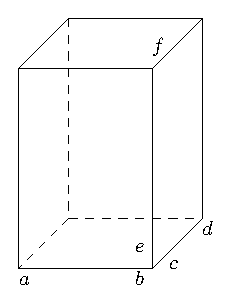
\includegraphics[width=4cm]{img/finiti/rettangolo.eps}
  \end{multicols}
  Il prodotto cartesiano $I_n*I_n*I_k$ individua il generico subparallelepipedo $V_{n,m,k}$.
\end{defi}
\clearpage
Definisco le somme di Riemann: $\sum f(x,y,z)*misV_{n,m,k}$\footnote{$misV_{n,m,k}$: misura il
  volume del parallelepipedo}\\
All'infittirsi delle decomposizioni le somme di Riemann convergono ad uno stezzo valore, tale
valore è definito {\color{red}integrale triplo} di $f(x,y,z)$ in $V$
\begin{equation*}
  \lim_{m\to \infty\text{ } n \to \infty \text{ } k\to \infty}\sum f(x,y,z) misV_{n,m,k}=\iiint_V f(x,y,z)dxdydz
\end{equation*}
Oppure, definisco le somme inferiore e le somme superiori
\begin{equation*}
  \begin{matrix}
    \text{Somme inferiori} &\sum misV_{n,m,k}*\min_{V_{n,m,k}}f(x,y,z)\\
    \text{Somme superiori} &\sum misV_{n,m,k}*\max_{V_{n,m,k}}f(x,y,z)
  \end{matrix}
\end{equation*}
All'infittirsi della decomposizione le somme inferiori crescono mentre le somme superiori
decrescono. Se convergono ad una stesso valore, tale valore è definito {\color{red}integrale triplo}
di $f(x,y,z)$ in $V$
\begin{equation*}
  \lim s(f,V)= \lim S(f,V)= \iint_V f(x,y,z) dxdydz
\end{equation*}
\subsection{Formule di riduzione per gli integrali tripli}
Sia $g(x,y)$ integrabile in un dominio normale $V$
\begin{equation*}
  \begin{matrix}
    V=\begin{cases}
        \alpha (x,y) \leq z\leq \beta (x,y)\\
        (x,y)\in D
      \end{cases} & \iiint_V f(x,y,z) dxdydz = \iint_D dxdy \displaystyle\int_{a(x,y)}^{\beta (x,y)} f(x,y,z)dz
  \end{matrix}
\end{equation*}
Se il dominio $D$ è normale rispetto all'asse $x$
\begin{equation*}
	V=\begin{cases}
		a\leq x\leq b\\
		g_1(x)\leq y\leq g_2(x)\\
		\alpha (x,y) \leq z \leq \beta (x,y)
	\end{cases} \iiint_V f(x,y,z) dxdydz = \int_\theta^\theta dx
	\int_{f_1(x)}^{f_2(x)}dy\int_{\alpha(x,y)}^{\beta(x,y)}f(x,y,z)dz
\end{equation*}
Se il dominio $D$ è normale rispetto all'asse $y$
\begin{equation*}
	V=\begin{cases}
		c\leq y \leq d\\
		h_1(y)\leq x \leq h_2(y)\\
		\alpha (x,y) \leq z \leq \beta(x,y)
	\end{cases} \iiint_V f(x,y,z) dxdydz = \int_c^d dy
	\int_{h_1(y)}^{h_2(y)}\int_{a(x,y)}^{\beta(x,y)} f(x,y,z) dz
\end{equation*}
Se il dominio $D$ è polarmente normale
\begin{equation*}
	V=\begin{cases}
		\theta_1\leq \theta \leq \theta_2\\
		\varphi_1(\theta)\leq \varphi \leq \varphi_2(\theta)\\
		\alpha (\varphi,\theta)\leq z \leq \beta(\varphi,\theta)
	\end{cases} \iiint_V f(x,y,z)dxdydz=\int_{\theta_1}^{\theta_2}d\theta
	\int^{\varphi_2(\theta)}_{\varphi_1(\theta)} \varphi d \varphi
	\int^{\beta(\varphi, \theta)}_{\alpha (\varphi,\theta)}
	f(\varphi,\theta,z)dz 
\end{equation*}
\begin{equation*}
	\begin{matrix}
		\alpha(x,y)&\to&\alpha (\varphi, \theta)\\
		\beta (x,y)&\to& \beta(\varphi, \theta)\\
		f(x,y,z) &\to & f(\varphi,\theta, z)\\
		dxdydz &\to & pd\theta d\varphi dz
	\end{matrix}
\end{equation*}
\clearpage
\subsection{Significato geometrico degli integrali}
\begin{equation*}
	\begin{matrix}
		\int & \text{area}\\
		\iint & \text{volume}\\
		\iiint & \text{nessun significato geometrico}
	\end{matrix}
\end{equation*}
\subsection{Coordinate polari e coordinate cilindriche}
$(x,y) \to (\varphi,\theta)$
\begin{equation*}
	\begin{matrix}
		\begin{cases}
			x=\varphi \cos \theta\\
			y=\varphi \sin \theta
		\end{cases} & \varphi =\sqrt{x^2+y^2} &det J=\varphi
	\end{matrix}
\end{equation*}
\paragraph{coordinate alindriche}
$(x,y,z)\to (\varphi,\theta,z)$
\begin{equation*}
	\begin{matrix}
		\begin{cases}
			x=\varphi \cos \theta\\
			y=\varphi \sin \theta\\
			z=z
		\end{cases} & \varphi =\sqrt{x^2+y^2+z^2} &det J=\varphi
	\end{matrix}
\end{equation*}
\paragraph{coordinate sferiche}
\begin{equation*}
	\begin{matrix}
		\begin{cases}
			x=\varphi \sin\theta \cos \alpha\\
			y=\varphi \sin \theta \sin \alpha\\
			z=\varphi \cos\theta
		\end{cases} 
	\end{matrix}
\end{equation*}
\subsection{Interazione per fette}
Considera un volume $V$ e lo interseco con un piano $z=k$. Così ottengo una
sezione $S_z$
\begin{equation*}
	z=1-x^2-y^2
\end{equation*}
Al variare di $z$ tra due valori, cioè facendo variare $S_z$ in funzione di $z$
descrivo il volume $V$.
\begin{esempio}
	\begin{equation*}
		\int_{0}^{1} S_zdz
	\end{equation*}
	$S_z$ è un cerchio di raggio $R(z)$ che depende da $z$
	\begin{equation*}
		\begin{matrix}
			z=1-x^2+y^2 & x^2+y^2=1-z\\
			R^2=1-z & R(z)=\sqrt{1-z}
		\end{matrix}
	\end{equation*}
	$S_z=\pi R^2=\pi(1-z)$
	\begin{equation*}
		\iint_T f(x,y,z)dxdydz=\int_0^1\pi(1-z)dz
	\end{equation*}
\end{esempio}
\subsection{Integrali curvilinei}
\subsubsection{Curve in $R^2$ e in $R^3$}
\begin{defi}
	Si definisce {\color{red}curva} una coppia del tipo $(\gamma,\Gamma)$ con
	\begin{equation*}
		\vec{F}(t)=(x(t),y(t),z(t),\dots) \text{ } t\in [a,b]
	\end{equation*}
	si tratta di un'applicazione $R\to R^n$ ad un valore di $t$ associo $n$
	valori\\
	Le curve possono essere:
	\begin{itemize}
		\item In forma cartesiana $\begin{matrix}
				z=f(x,y) &(R^3) \\
				y=f(x) &(R^2)
		\end{matrix} \begin{cases}
			x=t\\
			y=f(t)
		\end{cases}$
		\item In forma polare $\begin{matrix}
			\varphi =\varphi(\theta)&\varphi=2r\cos\theta & 0\leq \theta \leq 2\pi
	\end{matrix}$
		\item In forma parametrica $\begin{cases}
			x=x(t)\\
			y=y(t)\\
			z=z(t)
		\end{cases}$
	\end{itemize}
	Nello spazio una curva è l'intersezione tra due superfici.\\
	Ogni curva ha anche un {\color{red}sostegno}, che è il suo grafico nek
	piano o nello spazio.\\
	Una curva si definisce {\color{red}chiusa} se
	\begin{equation*}
		\begin{matrix}
			\vec{F}(t)=\begin{cases}
				x=x(t)\\
				y=y(t)
			\end{cases} & t\in [a,b]\text{ se } \vec{F}(a)=\vec{F}(b) &
			\begin{matrix}
				x(a)=x(b)\\
				y(a)=y(b)
			\end{matrix}
		\end{matrix}
	\end{equation*}
	\begin{figure}[ht]
		\centering
		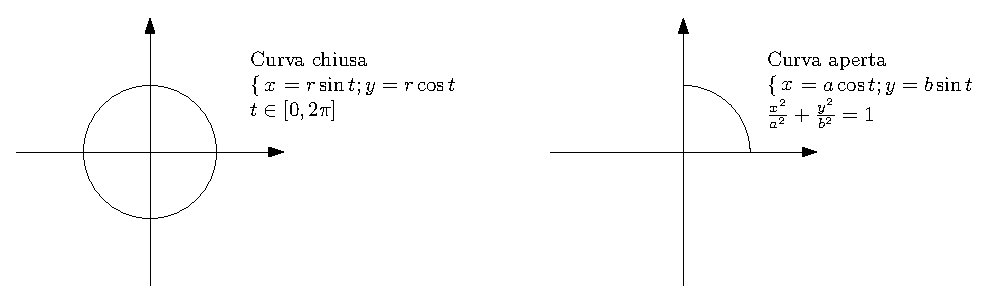
\includegraphics[width=13cm]{img/finiti/curva_chiusa_e_aperta.eps}
		\caption{Differenza tra curva chiusa e aperta}
	\end{figure}\\
	Una curva chiusa la {\color{red}frontiera} di un dominio
	\begin{multicols}{2}
		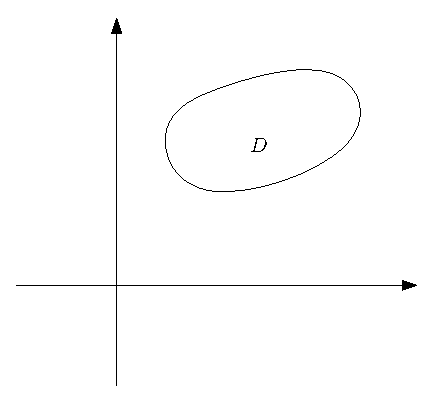
\includegraphics[width=6cm]{img/finiti/dominio.eps}\\
		\begin{equation}
			FD:\begin{cases}
				x=x(t)\\
				y=y(t)
			\end{cases} t\in [a,b]
		\end{equation}
	\end{multicols}
	Una curva si devinisce {\color{red}semplice} se presi due qualunque
	$t_1\neq t_2$ rusylta $\vec{F}(t_1)\neq \vec{F}(t_2)$ cioè 
	\begin{equation*}
		\begin{cases}
			x(t_1)\neq x(t_2)\\
			y(t_1)\neq y(t_2)\\
			z(t_1)\neq z(t_2)
		\end{cases}
	\end{equation*}
	Curva semplice $\gamma \begin{cases}
		x=t\\
		y=\sqrt{t}
	\end{cases} y=\sqrt{x}$ $\gamma \begin{cases}
		x=t\\
		y=t^2
	\end{cases} y=x^2$ Curva non semplice\footnote{$t_1\neq t_2$ ho due stessi
	valori della curva}\\
	Una curva è {\color{red}regolare} se è di classe $c^1$ e le sue derivate
	prime non sono mai nulle contemporaneamente
	\begin{equation*}
		\vec{F}(t)=\begin{cases}
			x=x(t)\\
			y=y(t)\\
			z=z(t)
		\end{cases}
		\begin{matrix}
			\vec{F}(t)\in c^\prime \\
			t\in[a,b]
		\end{matrix}
		r^\prime(t)=(x^\prime,y^\prime,z^\prime(t)\dots)\neq(0,0,0\dots)
	\end{equation*}
	Curva regolare
	\begin{equation*}
		\begin{matrix}
			\gamma z(t)=\begin{cases}
				x=t^3-t\\
				y=t^2-1
			\end{cases} & f\in [-1,1] & z^\prime(t) =\begin{cases}
				x^\prime(t)=3t^2-1\\
				y^\prime(t)=2t
			\end{cases} &\begin{matrix}
				\text{non sono mai nulle}\\
				\text{contemporaneamente}
			\end{matrix}
		\end{matrix}
	\end{equation*}
	\begin{multicols}{2}
		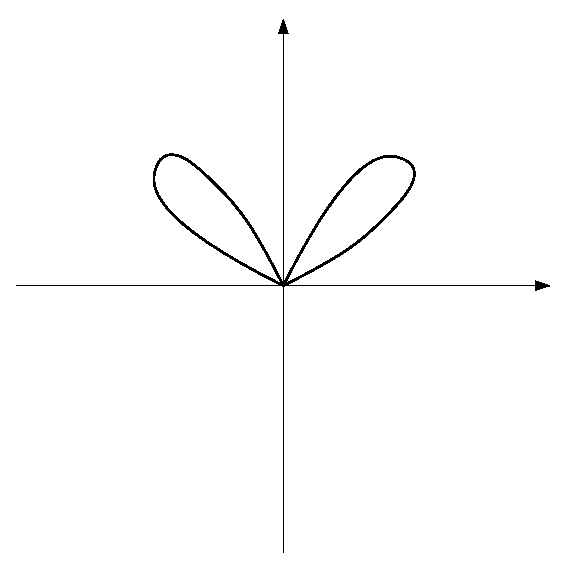
\includegraphics[width=6cm]{img/finiti/curva_regolare.eps}\\
		\begin{equation*}
			r(t)=\begin{cases}
				x=t(1-t^2)^2\\
				y=t^2(1-t^2)
			\end{cases} t\in[-1,1]
		\end{equation*}
	\end{multicols}
	Una curva è {\color{red}regolare a tratti} se è l'unione di curve regolari
	\begin{equation*}
		\gamma r(t)=\begin{cases}
			x=t^3\\
			y=t^2
		\end{cases} t\in[-1,1] \text{ in $x=0$ c'è una cuspide perciò non è regolare $y=\sqrt[3]{x^2}$}
	\end{equation*}
	$r(t)$ può però essere vista come l'unione di che curve regolari
	\begin{equation*}
		\gamma^\prime r (t)=\begin{cases}
			x=t^3\\
			y=t^2
		\end{cases} t\in [-1,0]
	\end{equation*}
	\begin{equation*}
		\gamma^{\prime\prime} r^{\prime\prime}=\begin{cases}
			x=t^3\\
			y=t^2
		\end{cases} t\in [0,1]
	\end{equation*}
	sostegno nel II quadrante
	\begin{equation*}
		\gamma=\gamma^\prime \vee \gamma^{\prime\prime}
	\end{equation*}
\end{defi}
\subsection{Lunghezza di una curva}
\begin{defi}
	Sia la curva $\gamma$ di equazione $\vec{F}(t)$, essa si definisce
	{\color{red}rettificabile} se esiste finito l'estremo superiore della
	poligonale $L(p)$ al variare della decomposizione.
	\begin{equation}
		sup_DL(\Delta)
	\end{equation}
	Suddivido la curva in tanti segmenti che formano la poligonale $L(D)$.
	All'infittirsi la poligonale approssimo sempre seguo la lunghezza della
	curva.\\
	Se la curva $\vec{F}(t)$ è di classe $c^1$ allora essa è
	{\color{red}rettificabile}
	\begin{equation}
		\vec{F}(t)=\begin{cases}
			x=x(t)\\
			y=y(t)\\
			z=z(t)
		\end{cases} t\in [a,b]
	\end{equation}
	e la sua lunghezza vale
	$L=\int_{a}^{b}\sqrt{[x^\prime(t)]^2+[y^\prime(t)]^2 + [z(t)]^2+\dots dt}$
\end{defi}
\subsection{Lunghezza di una curva in forma cartesiana}
Se la curva $\gamma$ nella forma $\begin{cases}
	x=t\\
	y=f(t)
\end{cases} t\in [a,b]$ ha come sostegno il grafico di $y=f(x)$\\
La lunghezza della curva è $L_\gamma=\int_{a}^{b}\sqrt{1+[f^\prime(x)]^2}dx$
\subsection{Lunghezza di una curva polare}
Se le curve è nella forma 
\begin{equation*}
	\begin{cases}
		e=e(\theta)\\
		\theta_1\leq\theta\leq\theta_2
	\end{cases} 
\end{equation*}
La sua lunghezza vale: 
\begin{equation*}
	L_\gamma
	=\int_{\theta_1}^{\theta_2}\sqrt{\varphi^2(\theta)+[\varphi^\prime(\theta)]^2}
	d\theta
\end{equation*}

